\documentclass[spanish]{beamer}

\include{conf/preconfig}
\include{conf/packages}
\include{conf/config}
\include{beamerconf}
%
%
\usetheme{Bergen}
\usecolortheme{orchid}
%
%
%
\title{Identificación de edificios y monumentos a partir de fotografías tomadas 
con dispositivos móviles}
\author{Esteban C. Fornal \and Christian N. Pfarher \and Mauro J. Torrez}
\date{\today}

\begin{document}
%
\frame{\titlepage}

\section[Outline]{Objetivo}

\begin{frame}{}
\frametitle{Objetivo}
Identificar edificios y monumentos a partir de fotografías
\end{frame}

\section[Outline]{Herramientas}
\begin{frame}{Dos técnicas:}
\begin{itemize}
\item<1-> Transformada de Hough
\item<2-> Histograma
\end{itemize}
\end{frame}

\begin{frame}{Transformada de Hough}
  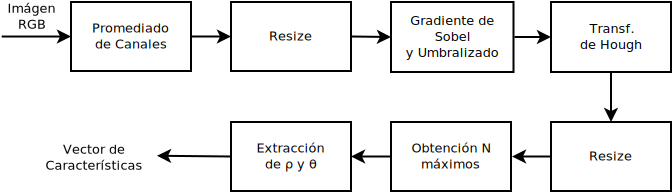
\includegraphics[width=9cm]{../diagramas/procesohough}
\end{frame}


\begin{frame}{Histograma}
  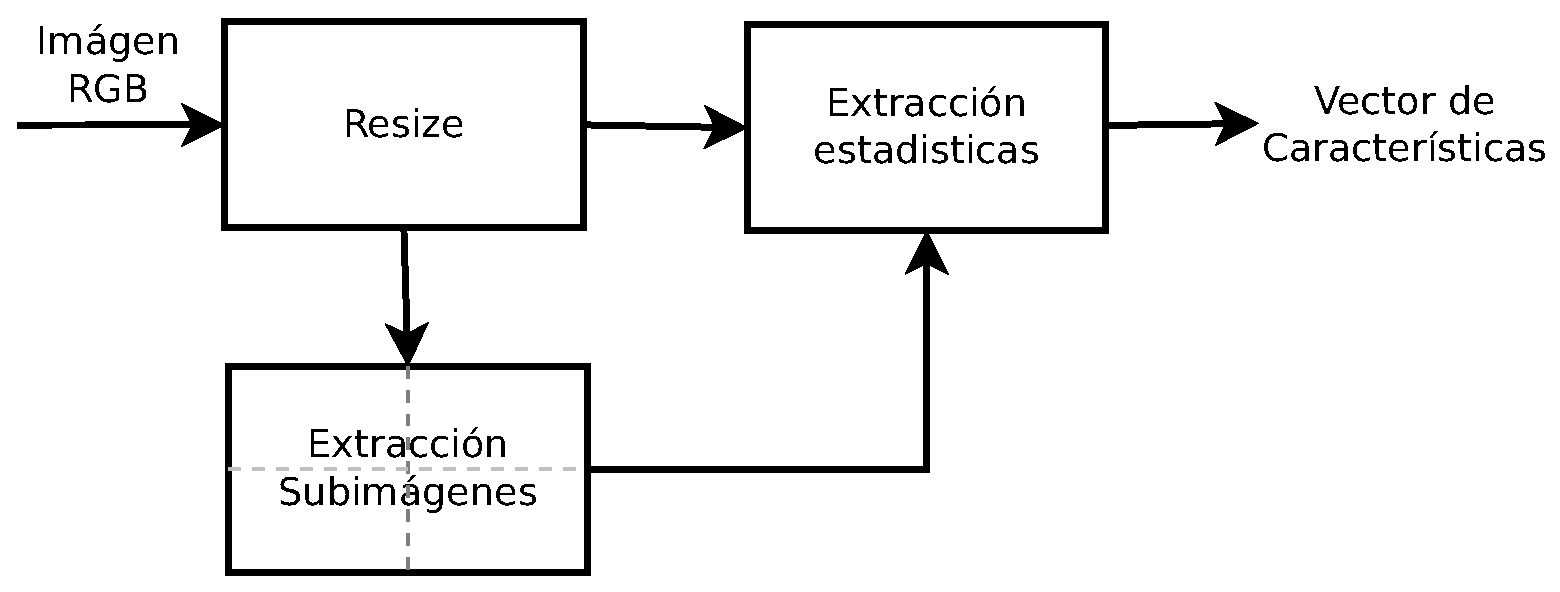
\includegraphics[width=9cm]{../diagramas/procesoestadisticas}
\end{frame}


\begin{frame}{Método}
  \begin{itemize}
  \item ambas tecnicas !!!bla
  \end{itemize}
\end{frame}

\begin{frame}{Pruebas}
  \begin{align*}
    MSE = \frac{1}{MN} \sum_x\sum_y [ f(x,y) - g(x,y) ]^{2}
  \end{align*}
\end{frame}


\begin{frame}{Resultados}
  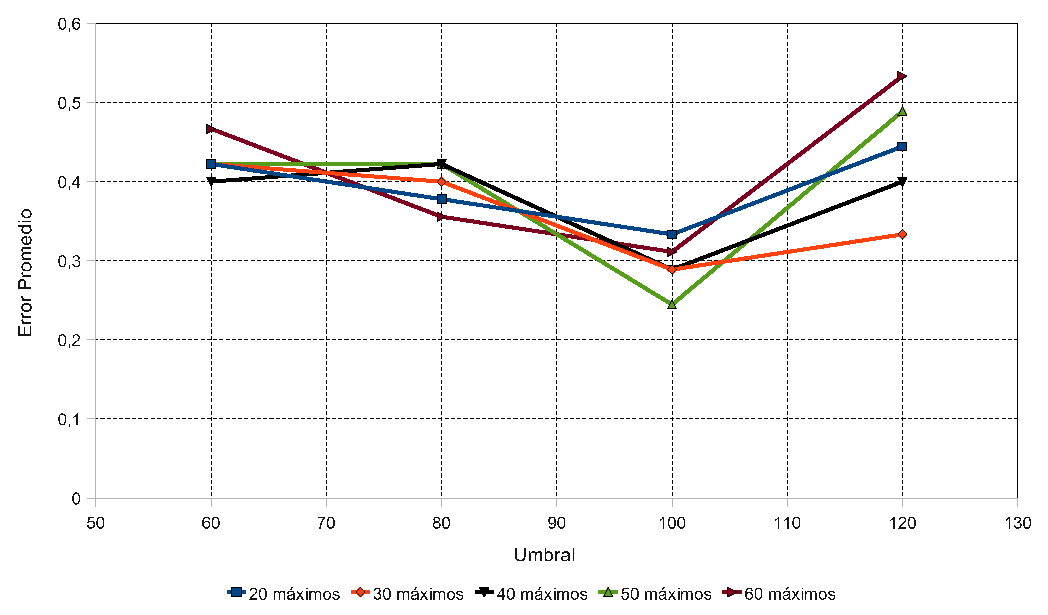
\includegraphics[width=9cm]{../diagramas/estadistica_noche_iguales}
\end{frame}

\begin{frame}{Resultados}
  \begin{itemize}
  \item Sensores
    \begin{itemize}
    \item Cantidad
    \item Tipo
    \item Configuración
    \end{itemize}
  \item Resultados satisfactorios para la información disponible
  \end{itemize}
\end{frame}

\begin{frame}{Conclusiones}
  \begin{itemize}
  \item Sensores
    \begin{itemize}
    \item Cantidad
    \item Tipo
    \item Configuración
    \end{itemize}
  \item Resultados satisfactorios para la información disponible
  \end{itemize}
\end{frame}

\end{document}








